\chapter{Grundlagen}\label{chap:Grundlagen}
\section{Bevölkerungsdichte}
Die Bevölkerungsdichte eines Gebietes $\rho_{Gebiet}$ wird berechnet, indem die Anzahl der Einwohner im Gebiet $n_{Einwohner\ Gebiet}$ durch die Fläche des Gebiets $A_{Gebiet}$ geteilt wird:
\begin{equation}\label{eq:Bevölkerungsdichte}
    \rho_{Gebiet} = \frac{n_{Einwohner\  Gebiet}}{A_{Gebiet}}
\end{equation}
\section{7-Tages Inzidenz}\label{sec:Datenaufbereitung}
Die 7-Tages Inzidenz $i_t$ wird für jeden Tag $t$ seit Beginn der Pandemie berechnet.
Zuerst wird von der akkumulierte Zahl der Fälle am gewählten Tag $f_t$ die akkumulierte Zahl der Fälle am siebten Tag vor dem jeweiligen Tag $f_{t-7}$ abgezogen, dies ergibt die neu hinzugekommenen Fälle innerhalb von sieben Tagen.
Diese Zahl wird durch die Anzahl der Bewohner des Gebiets $p$ geteilt und mit 100.000 multipliziert. Dies ergibt \autoref{eq:7-Tages_Inzidenz}.
\begin{equation}\label{eq:7-Tages_Inzidenz}
    i_t= \frac{f_t-f_{t-7}}{p}\cdot 100.000
\end{equation}
Wie in \autoref{fig:neue_Fälle_pro_Wochentag_Deutschland} klar zu sehen, werden an Wochenenden im Schnitt deutlich weniger neue Fälle registriert als an den anderen Wochentagen.
Daher werden immer sieben Tage in der 7-Tages Inzidenz zusammengefasst.
\begin{figure}[H]
    \centering
    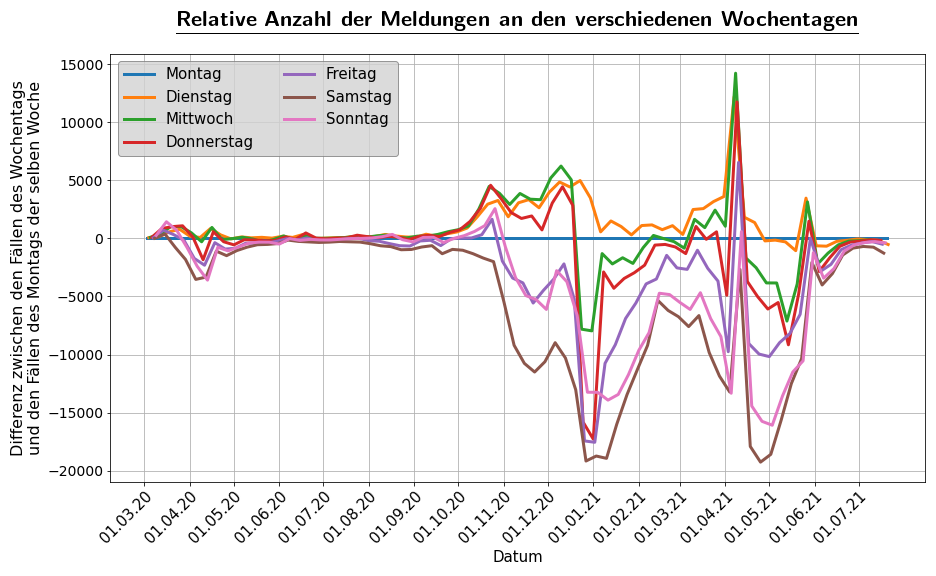
\includegraphics[width=0.95\textwidth]{figures/neue_Fälle_pro_Wochentag_Deutschland.png}
    \caption{In Deutschland neu gemeldete COVID-19 Fälle am jeweiligen Wochentag im Vergleich zu den am Montag der selben Woche gemeldeten Fälle.}
    \label{fig:neue_Fälle_pro_Wochentag_Deutschland}
\end{figure}
Da die Bevölkerung der deutschen Landkreise und Regierungsbezirke nicht identisch ist, wird jeweils durch die Bevölkerungszahl geteilt, um die einzelnen Gebiete miteinander vergleichen zu können.

Aufgrund der ansonsten sehr kleinen Zahlen, bietet es sich zudem an, das Ergebnis mit 100.000 zu multiplizieren.

\section{Susceptible-Infectious-Removed Modell}
Ein Weg zur Beschreibung der Pandemie bietet das SIR Modell \autocite{SIR}. Dieses Modell teilt die Mitglieder einer Menschengruppe in eine der drei folgenden Kategorie ein und ermöglicht es, die zeitliche Entwicklung einer Pandemie übersichtlich darzustellen:
\begin{itemize}
    \item \glqq{}susceptible\grqq{}: Menschen, welche angesteckt werden können.
    \item \glqq{}infectious\grqq{}: Infizierte Menschen, welche weitere Menschen anstecken können. Werden auch als "die aktiven Fälle" bezeichnet.
    \item \glqq{}recovered\grqq{}: Menschen, welche in die Kategorie \glqq{}infectious\grqq{} fielen und\\
    nun immun gegen die Krankheit sind. (Hierzu zählen auch Verstorbene)
\end{itemize}


\section{Korrelationsanalyse mithilfe einer Faltung}\label{sec:BeschreibungKorrelationsanalyse}
\subsection{Berechnung der Korrelationswerte}\label{Grundlagen:Berechnung der Korrelationwerte}
Um festzustellen, ob die 7-Tages-Inzidenzen einiger Landkreise im Vergleich zu anderen Landkreisen eher voraus- oder nacheilen, wird in diesem Fall die Korrelationsfunktion verwendet \autocite{Korrelation}.

Bei diskreten Werten, aufgeteilt in zwei Zeitserien $X$ und $Y$, wie in diesem Fall, lässt sich eine Faltung sehr einfach umsetzen:
Für eine zeitliche Verschiebung $\tau$ wird mit jedem Wert $x_i$ zum jeweiligen Zeitpunkt $t_i$ aus der ersten Zeitserie mit dem zugehörigen Wert $y_i$ aus der zweiten Zeitserie ein Produkt gebildet. Der zugehörige Wert aus der zweiten Zeitserie entspricht hierbei dem Zeitpunkt $t$ des Wertes der ersten Zeitserie plus die gewählte Verschiebung $\tau$. Sollte dieser zweite Wert nicht existieren, wird kein Produkt gebildet.

Für jede zeitliche Verschiebung $\tau$, für die mindestens ein Produkt gebildet wird, werden alle möglichen Produkte aufsummiert.

Somit ergibt sich \autoref{eq:Korrelation}, mit $n := $ Länge von $X$ und wenn $y_{i+\tau} \not\in Y$, dann $y_{i+\tau} := 0$:
\begin{equation}\label{eq:Korrelation}
    c(\tau) = \sum_{i=1}^n x_i\cdot y_{i+\tau}
\end{equation}


Bildlich gesprochen wird die zweite Zeitserie an der ersten Zeitserie vorbeigeschoben, beginnend an dem Punkt, an dem ausschließlich das erste Element der ersten Zeitserie mit dem letzten Element der zweiten Zeitserie multipliziert wird. Dies ist beispielhaft mit den Folgen $[1,2,3,2]$ und $[5,7,5,1]$ in \autoref{fig:Korrelation Beispiel} dargestellt.

\begin{figure}[H]
    \centering
    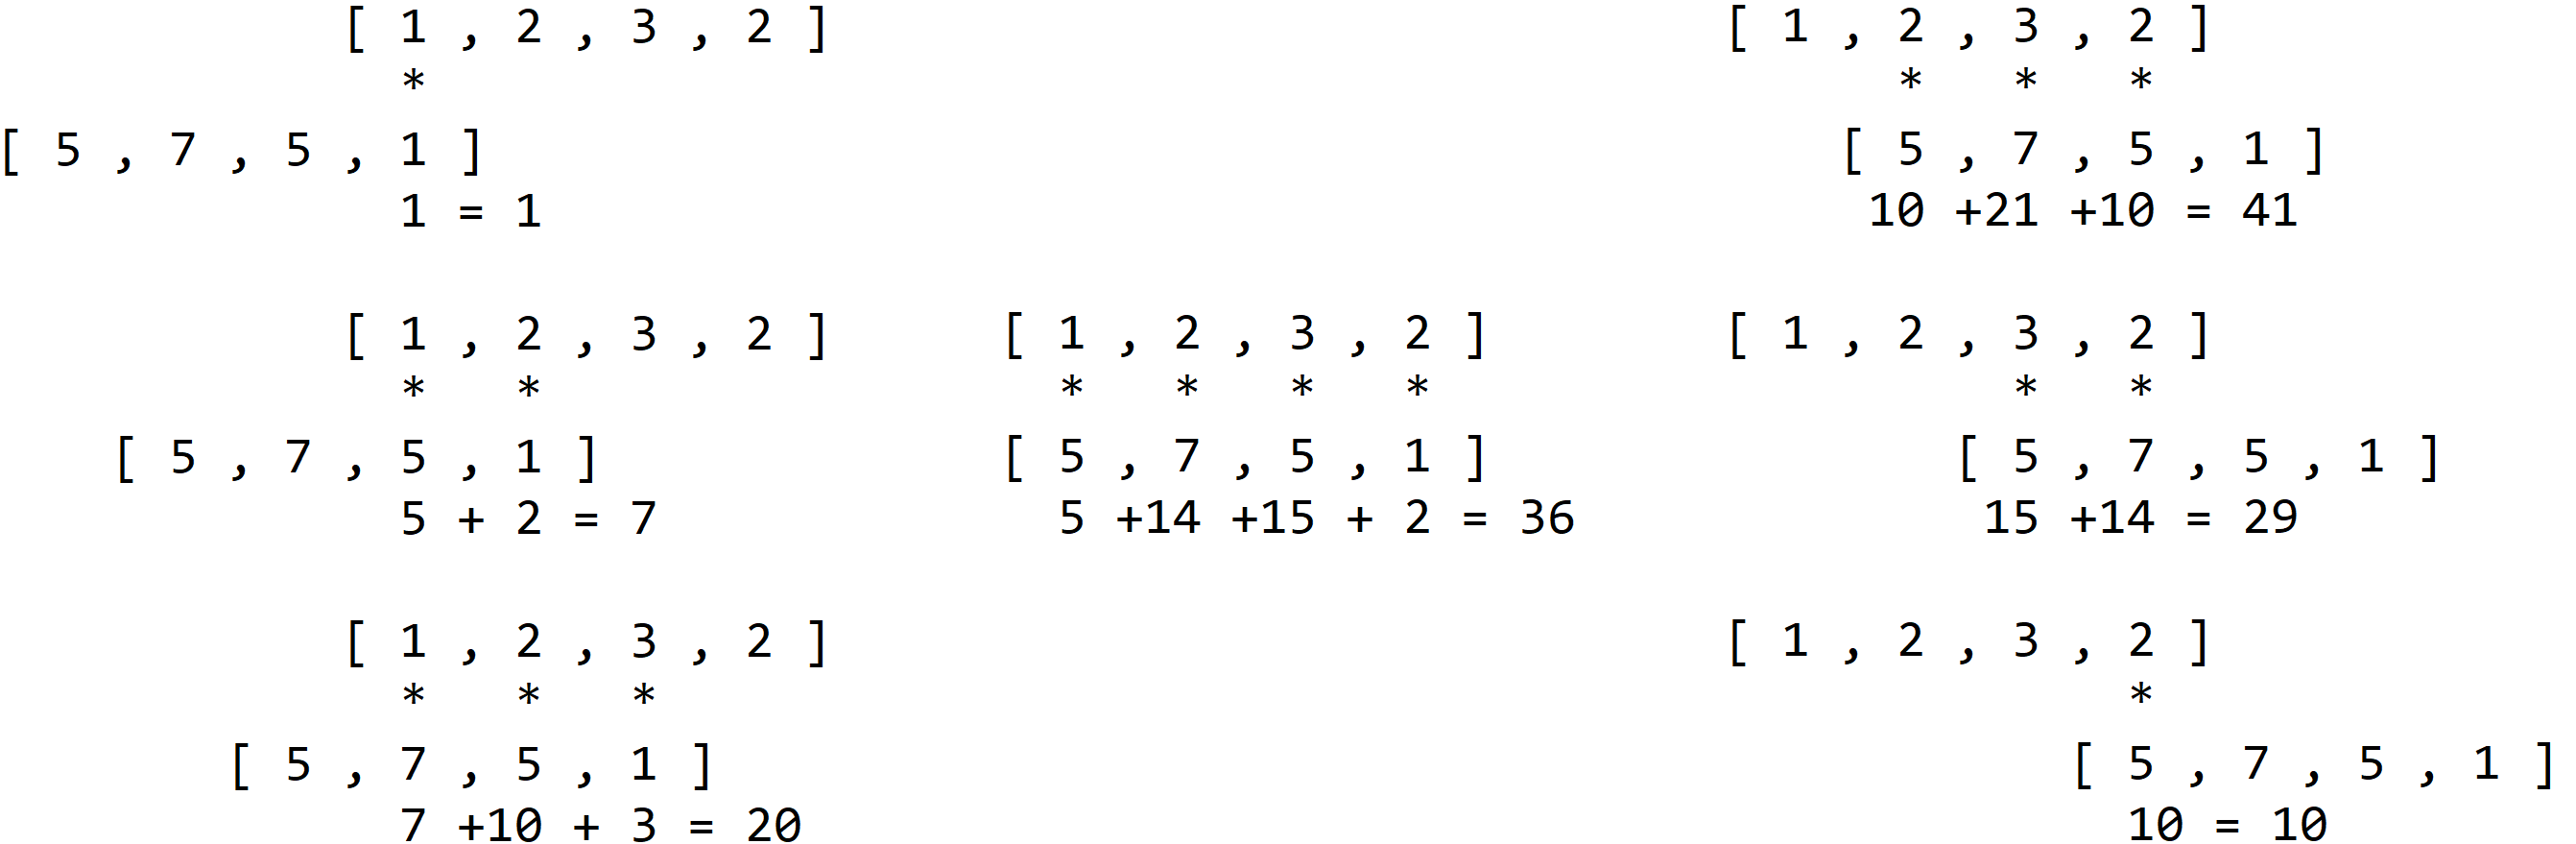
\includegraphics[width=\textwidth]{figures/Korrelation.png}
    \caption{Beispielhafte Darstellung einer Faltung anhand der Folgen $[1,2,3,2]$ und $[5,7,5,1]$. Auf der linken Seite hinter dem Gleichheitszeichen von oben nach unten die Korrelationswahrscheinlichkeiten für die negativen Verschiebungen $\tau=-3$, $\tau=-2$ und $\tau=-1$. Entsprechend in der Mitte bei keine Verschiebung ($\tau=0$) und rechts für die positiven Verschiebungen $\tau=1$, $\tau=2$ und $\tau=3$}
    \label{fig:Korrelation Beispiel}
\end{figure}

Da in diesem Beispiel jedoch die Landkreise mit höheren Werten scheinbar eine größere Korrelation aufweisen und die kleineren Verschiebungen übergewichtet werden, da ihre Summe aus mehr Produkten besteht, müssen die Werte, wie in \autoref{eq:skalierte_Korrelation}, noch skaliert werden.
Um die Landkreise mit allgemein größeren Werte anzupassen, wird durch die Korrelation mit keiner zeitlichen Verschiebung zu sich selbst
geteilt, somit ergibt sich mit den neuen Werten immer bei einer Korrelationsanalyse mit sich selbst immer ein Wert von eins bei keiner zeitlichen Verschiebung.
\begin{equation}\label{eq:skalierte_Korrelation}
    c(\tau) =\sum_{i=1}^n \frac{x_i}{\sqrt{\sum_{j=1}^n x_j^2}}
    \frac{y_{i+\tau}}{\sqrt{\sum_{j=1}^n y_j^2}}= 
    \frac{\sum_{i=1}^n x_i\cdot y_{i+\tau}}{\sqrt{\sum_{i=1}^n x_i^2}\sqrt{\sum_{i=1}^n y_i^2}}
\end{equation}

Da bei der Faltung bei größeren Verschiebungen zudem weniger Produkte aufsummiert werden, muss bei jeder Summe durch die Anzahl der aufsummierten Produkte geteilt werden. Da jede Zeitserie gleich lang ist, in diesem Fall $n$ Elemente, ergibt sich \autoref{eq:skalierte_Korrelation_geteilt_durch_Produkte}, wobei die Anzahl der Produkte $m$ der Länge der Zeitserie $n$ minus den Betrag der Verschiebung $\vert\tau\vert$ entspricht:
\begin{equation}\label{eq:skalierte_Korrelation_geteilt_durch_Produkte}
    c(\tau) =\frac{n}{m} \frac{\sum_{i=1}^n x_i\cdot y_{i+\tau}}{\sqrt{\sum_{i=1}^n x_i^2}\sqrt{\sum_{i=1}^n y_i^2}}=
    \frac{n}{n-\vert\tau\vert} \frac{\sum_{i=1}^n x_i\cdot y_{i+\tau}}{\sqrt{\sum_{i=1}^n x_i^2}\sqrt{\sum_{i=1}^n y_i^2}}
\end{equation}

Zudem wird von jedem Wert der Zeitserie $x_i$ der Mittelwert $\overline x = \frac{1}{n}\sum_{i=1}^n x_i$ abgezogen, dadurch lassen sich Antikorrelationen feststellen: Wenn beispielsweise die Anzahl der COVID-19 Infektionen eines Landkreises zu einem Zeitpunkt überdurchschnittlich schnell wächst, also die 7-Tages-Inzidenz minus den Mittelwert der 7-Tages-Inzidenzen positiv ist, und das andere Edukt aus der anderen Zeitserie negativ ist, also in dem anderen Landkreis die Anzahl der COVID-19 Infektionen unterdurchschnittlich schnell wächst, ergibt sich ein negatives Produkt, da die Situation in dem einen Landkreis verhältnismäßig ruhig wirkt, während die Situation im anderen Landkreis schneller als üblich kritisch wird. Ergibt die Summe aus all den Produkten einer Faltung eine negative Zahl, scheint die 7-Tages Inzidenz des einen Landkreises langsam zu steigen, während die 7-Tages Inzidenz des anderen Landkreises schnell zu steigen scheint, dies wird hier Antikorrelation genannt.

Mit allen Ergänzungen berechnet sich die Korrelation $c(\tau)$ zwischen zwei Zeitserien $X:|X|=n$ und $Y:|Y|=m$ mit einer Verschiebung $\tau$ relativ zu $X$ aus den einzelnen Werten $x_i\in X$, $y_i \in Y$ und den Mittelwerten der Zeitserien $\overline x,\ \overline y$ wie in \autoref{eq:komplette_skalierte_Korrelation} beschrieben.
\begin{equation}\label{eq:komplette_skalierte_Korrelation}
    c(\tau) =\frac{n}{m}
    \frac{\sum_{i=1}^n (x_i-\overline x)\cdot (y_{i+\tau}-\overline y)}{\sqrt{\sum_{i=1}^n (x_i-\overline x)^2}\sqrt{\sum_{i=1}^n (y_i-\overline y)^2}}
\end{equation}
\todo{Quelle}

\subsection{Korrelation zwischen zwei Gebieten am Beispiel von Flensburg und Kiel}
Um die hergeleiteten Gleichungen und die weiterhin verwendete Terminologie zugänglicher zu machen, wird eine Korrelationsanalyse mit dem Verlauf der 7-Tages Inzidenz der Stadtkreise Flensburg und Kiel durchgeführt. Der Verlauf der 7-Tages Inzidenz der beiden Stadtkreise sind in \autoref{fig:Inzidenz_Flensburg} und \autoref{fig:Inzidenz_Kiel} einmal im Original und einmal um die mittlere 7-Tages Inzidenz in x-Richtung verschoben abgebildet.

\begin{figure}[H]
    \centering
    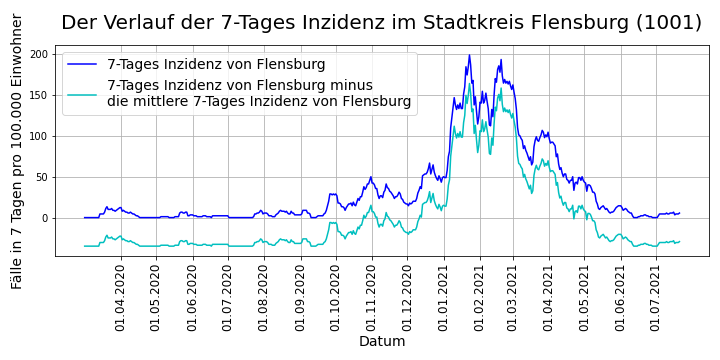
\includegraphics[width=0.95\textwidth]{figures/Inzidenz_Flensburg.png}
    \caption{Der Verlauf der 7-Tages Inzidenz des Stadtkreises Flensburg (Gemeindeschlüssel 1001).}
    \label{fig:Inzidenz_Flensburg}
\end{figure}
In \autoref{fig:Inzidenz_Flensburg}, \autoref{fig:Inzidenz_Kiel}, \autoref{fig:correlation_Flensburg_Kiel}, \autoref{fig:correlation_Flensburg_Kiel_scaled_autocorrelation} und \autoref{fig:correlation_Flensburg_Kiel_scaled_complete} ist das Ergebnis mit den originalen 7-Tages Inzidenzen blau dargestellt und das Ergebnis mit den 7-Tages Inzidenzen, von denen der Mittelwert der 7-Tages Inzidenzen des jeweiligen Landkreises abgezogen wurde, hellblau dargestellt.
\begin{figure}[H]
    \centering
    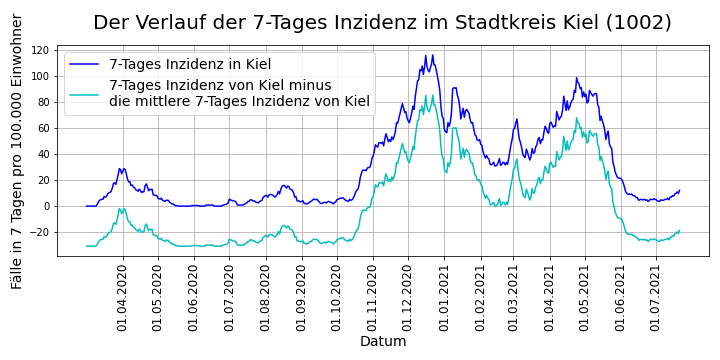
\includegraphics[width=0.95\textwidth]{figures/Inzidenz_Kiel.png}
    \caption{Der Verlauf der 7-Tages Inzidenz des Stadtkreises Kiel (Gemeindeschlüssel 1002).}
    \label{fig:Inzidenz_Kiel}
\end{figure}
In \autoref{fig:correlation_Flensburg_Kiel} ist die unskalierte Faltung, wie sie in \autoref{eq:Korrelation} definiert ist, abgebildet.
\begin{figure}[H]
    \centering
    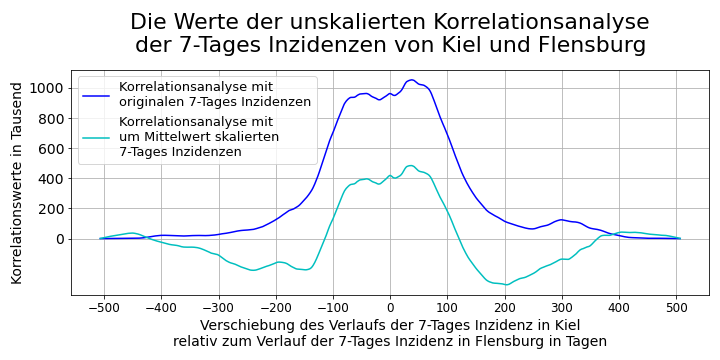
\includegraphics[width=0.95\textwidth]{figures/correlation_Flensburg_Kiel.png}
    \caption{Caption}
    \label{fig:correlation_Flensburg_Kiel}
\end{figure}
In \autoref{fig:correlation_Flensburg_Kiel_scaled_autocorrelation} ist die nach \autoref{eq:skalierte_Korrelation} um die Autokorrelation skalierte Faltung dargestellt.
\begin{figure}[H]
    \centering
    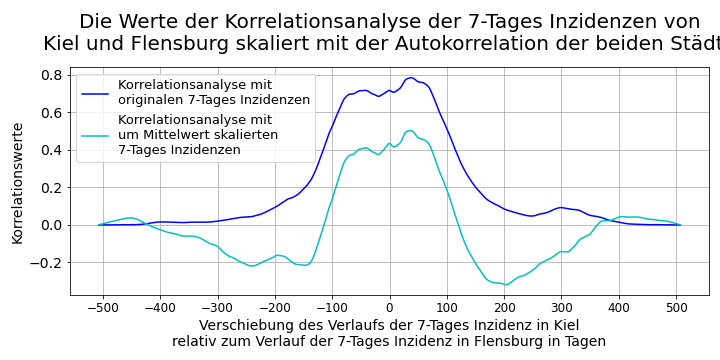
\includegraphics[width=0.95\textwidth]{figures/correlation_Flensburg_Kiel_scaled_autocorrelation.png}
    \caption{Caption}
    \label{fig:correlation_Flensburg_Kiel_scaled_autocorrelation}
\end{figure}
Wenn nach \autoref{eq:skalierte_Korrelation_geteilt_durch_Produkte} die  Summen jeweils durch die Anzahl ihrer Summanden (den Produkten) geteilt werden, ergibt sich \autoref{fig:correlation_Flensburg_Kiel_scaled_complete}.
\begin{figure}[H]
    \centering
    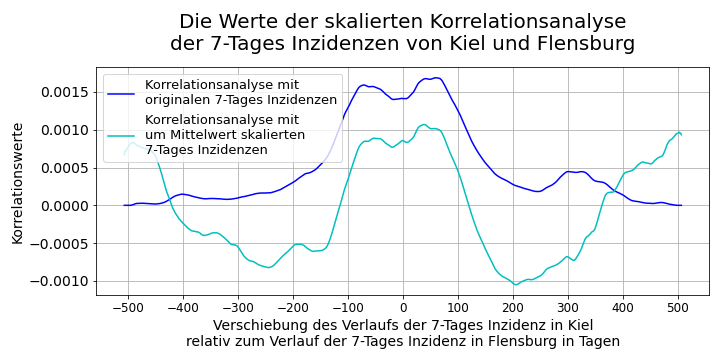
\includegraphics[width=0.95\textwidth]{figures/correlation_Flensburg_Kiel_scaled_complete.png}
    \caption{Caption}
    \label{fig:correlation_Flensburg_Kiel_scaled_complete}
\end{figure}

In \autoref{fig:correlation_Flensburg_Kiel_scaled_complete} ist schön zu erkennen, das die Korrelationsanalyse von zwei Zeitserien mit 508 7-Tages Inzidenzen 1015 Korrelationswerte ergibt.
Für jeden der 412 Landkreis ergeben sich daher aus der Korrelationsanalyse mit sich selbst und jedem anderen Landkreise 418.180 Werte, ebenso ergeben sich für jeden der 38 Regierungsbezirk 38.570. Dies ergibt in Summe $
%38.570\cdot 38 + 418.180\cdot412 =
1.465.660+172.290.160=173.755.820$ Werte.

Jeder Wert gibt die Wahrscheinlichkeit einer Korrelation bei der jeweiligen Verschiebung an, wobei die zugeordneten Verschiebungen von links nach rechts bei jedem Schritt um eins zunehmen und der mittlerste der Korrelationswerte der Verschiebung $\tau = 0$ zugeordnet ist. Die Verschiebung ist im Kontext dieser Arbeit stets in ganzen Tagen zwischen $-507$ und $507$ angegeben. Der Wert an Position 501 in der Liste der Korrelationswerte gibt also an, wie wahrscheinlich der Verlauf der 7-Tages Inzidenz des ersten Gebiets mit dem um eine Woche nach links verschobenen Verlauf der 7-Tages Inzidenz des zweiten Gebiets korreliert.


\subsection{Komprimierung und Darstellung als Matrizen}\label{sec:Grundlagen:Korrelation:Komprimierung}
Das Ziel der nachfolgend beschriebenen Schritte ist, die Korrelation von zwei Gebieten auf einen Wert zusammenzuführen, sodass man einfach und schnell alle Korrelationen zwischen zwei Gebieten vergleichen kann.

In dieser Arbeit werden nur Korrelationen mit einem zeitlichen Versatz zwischen $\tau=-50$ und $\tau=50$ betrachtet, da zum einen eine Interpretation für eine Verschiebung von mehr als 4 Wochen sehr schwierig ist und zum anderen einzelne Ausreißer bei größeren Verschiebungen stärker ins Gewicht fallen, weil immer weniger Produkte aufsummiert werden.
\todo{anderes Wort für schwierig in \glqq{}Interpretation für eine Verschiebung von mehr als 4 Wochen sehr schwierig ist\grqq{}}
Um ein detailliertes Bild zu erhalten, werden zudem Korrelationsanalysen für die Verschiebungen $\tau\in[-30,30]$ und $\tau\in[-14,14]$ durchgeführt.

Somit sind jeder Kombination aus zwei Landkreisen nur noch höchstens 101 Werte zugeordnet. Diese Werte werden in zwei verschiedenen Varianten zu einem Wert zusammengefasst:
\begin{itemize}
    \item Die Verschiebung mit dem maximalen Korrelationswert: Der maximale Wert wird herausgesucht und die zugehörige zeitliche Verschiebung wird als Maß dafür angegebenen, bei welcher Verschiebung in Tagen am wahrscheinlichsten eine Korrelation vorliegt.
    \item Die Verschiebungstendenz: Der Durchschnitt der ersten Hälfte der Liste wird vom Durchschnitt der zweiten Hälfte abgezogen. Das Resultat ermöglicht eine grobe Einschätzung, ob der maximale Wert nur ein Ausreißer ist oder nicht.
\end{itemize}
Die erste Variante generiert Werte welche sich leicht interpretieren lassen. Doch um die kompletten Informationen aus der Liste zu verarbeiten und nicht nur einen Wert herauszunehmen, bietet es sich an, das Ergebnis der ersten Variante mit dem der zweiten Variante zu vergleichen.
Jedoch lässt sich bei der zweiten Variante nur noch feststellen, ob die Werte der Zeitserie vor, nach oder mit den Werten der anderen wachsen, jedoch nicht mehr wie viele Tage früher/später - dafür braucht es das Ergebnis der ersten Variante.

Die Werte lassen sich jeweils in zwei Matrizen darstellen: Jeder Zeile und Spalte wird der Index für ein Gebiet zugeordnet und der Wert in einer Zelle entspricht dem Ergebnis der Korrelationsanalyse der Gebiete, denen jeweils der Index der Zeile und der Spalte zugeordnet ist.
Die Matrizen sind (mit verkehrtem Vorzeichen) symmetrisch an der Diagonalen von links oben nach rechts unten. Die Diagonalen sind mit Nullen besetzt, da die positive Verschiebung symmetrisch zur negativen Verschiebung ist und die Korrelation mit sich selbst trivialerweise bei einer Verschiebung von $\tau=0$ am größten ist, da die Werte und Trends komplett identisch sind.

Um den Landkreisen Werte zuzuordnen und nicht der Kombination aus Landkreisen, wird sowohl bei den Maximalwerten wie auch den Verschiebungstendenzen der Mittelwert gebildet, indem die Zeilen der Matrizen aufsummiert werden und durch die Anzahl der Spalten geteilt werden.
\section{Durchschnitt, Farbgebung und Skalierung}\label{sec:Durchschnitt, Farbgebung und Skalierung}
Um schnell verständliche Abbildungen bereitstellen zu können, werden die Werte skaliert und die Farbgebung der Deutschlandkarten derart angepasst, dass das gesamte Farbspektrum abgedeckt wird. Das Farbspektrum reicht gemäß den Farben des Regenbogens von blau über grün zu gelb zu rot, wie in \autoref{fig:color_schemes} demonstriert. Die niedrigsten Werte werden blau gefärbt.
Da manche dieser Farbwerte im Kontrast zu einem weißen Hintergrund schwer zu erkennen sind, ist der Hintergrund der meisten Abbildungen grau.

\begin{figure}
    \centering
    
\includegraphics[width=0.8\textwidth]{figures/color_schemes.png}
    \caption{Das Farbspektrum, in welchem sich die Darstellungen bewegen. Von links nach rechts steigen die eingegebenen Werte konstant. Der angegebene Wert wird jeweils anhand des ersten und des letzten Werten einer Referenzliste linear in diesem Spektrum verortet.}
    \label{fig:color_schemes}
\end{figure}

Die Matrizen werden durch die verwendete Programmbibliothek \glqq{}Matplotlib\grqq{} automatisch eingefärbt.


Um die Daten zusammenfassen wird das arithmetische Mittel benutzt. Der Mittelwert entspricht nach \autoref{eq:Mittelwert} der Summe der einzelnen Werte $x_1$, $x_2$, $x_3$ ... $x_n$ geteilt durch ihre Anzahl $n$.
\begin{equation}\label{eq:Mittelwert}
    \bar x = \frac{1}{n}\sum_{i=1}^n x_i
\end{equation}